

\section{Introduction}
\label{sec:ed:intro}

In this lab we will study the behavior of charges moving in uniform electric
and magnetic fields. We will discover that electrons in a uniform magnetic
field move in circular orbits, and we will determine the functional dependence 
of the path radius on both the strength of the magnetic field and the strength 
of the potential used to accelerate the electrons. Using these relationships we
will calculate the charge-to-mass ratio of the electron. 

This measurement of the electron charge-to-mass ratio is a great feat.  We 
cannot put a single electron on a scale to weigh it. There is however, another 
simple experiment, called the Millikan oil drop experiment, which determines 
the electric charge of a single electron.  From these two measurements, it is 
possible to calculate the mass of the electron; it is 
$9.109~389~7(57)\cdot 10^{-31}$ kg, a small number indeed.

We will also find that our relationship between the path radius, accelerating
potential, magnetic field strength, and charge-to-mass ratio will lead to 
having several beams of different path radii if we were to use particles of 
varying charges.  That is, if we were to send into our apparatus a beam 
containing particles with two distinct values of electric charge, the magnetic 
field would split the beam up, one species of particle would move in a circular
path of some radius, while the other would move in a circle of a different 
radius. We will be using only electrons in our beam for this experiment and we 
will find only one circular orbit in the magnetic field. We may deduce from 
this that all electrons have the same electric charge. This is also a result
of fundamental significance. 

\section{Theory}

\subsection{References}

Electric and magnetic fields are introduced in Serway, Chapter~23 (Electric 
Fields), and Chapter~29 (Magnetic Fields). Particularly 
relevant are the sections on the motion of charges in uniform fields:
Section~23.7 (Motion of Charged Particles in a Uniform Electric Field), 
 and Section~29.5 (Application of the Motion of a Charged Particle in a Magnetic Field).     

\subsection{The Physical Situation}

Consider the situation posed in Figure~\ref{fig:ed:elec}, where electrons 
(the $e^-$) are boiled off a hot filament, then accelerated through an 
electric potential $V$, and finally enter a region of uniform magnetic 
field~$\vec{B}$.
\begin{figure}[htb]
\centering \epsfxsize=10cm 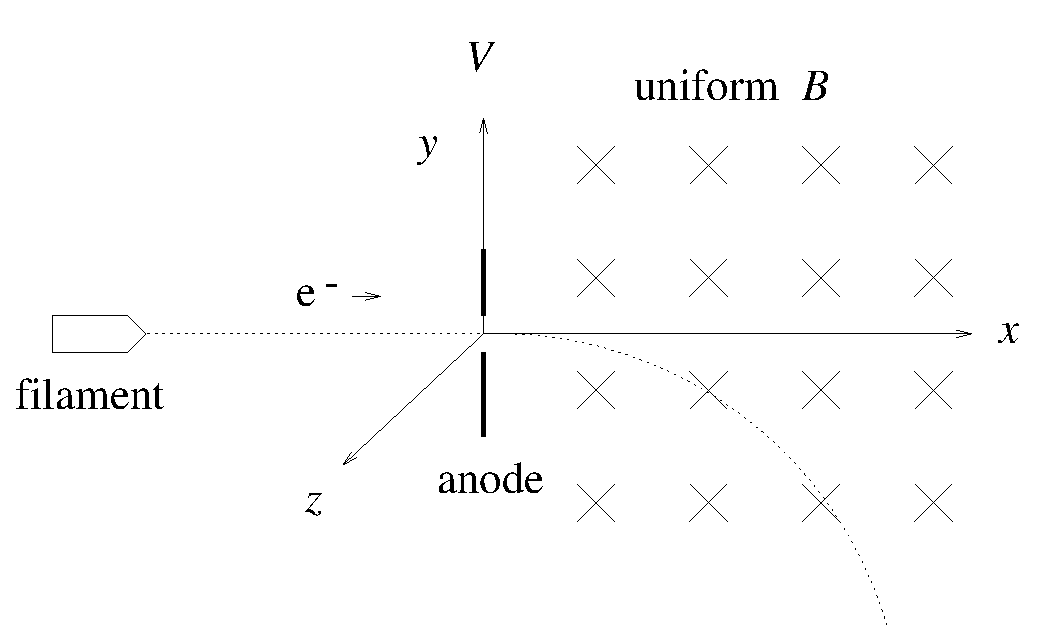
\includegraphics[scale=0.6]{3_electrondynamics/electron.eps}
\caption{The electron beam.}
\label{fig:ed:elec}
\end{figure}
The experimental apparatus we will use in the lab is designed to resemble this 
situation as closely as possible.
 
Let us assume that we may consider each electron independently. This is a big 
assumption, since we're neglecting any interaction between the electrons in 
our beam.  We know that electrons have like charges, so they should repel one
another. However, the accelerating potential and magnetic field in our 
apparatus are much stronger than this Coulomb interaction between pairs (or 
groups) of electrons.  Therefore, we're not really making a bad assumption by 
treating the electrons independently. We can also gain a bit more generality if
we forget for a while that we're actually dealing with electrons and we 
consider the more general situation of particles of some charge $q$ in the 
apparatus.  We can always get the specific result for the electron by taking 
$q=-e$. 

\subsection{Uniform Electric Field}

We know that a particle of charge $q$ and mass $m$ in a constant electric 
potential $V$ will accelerate linearly.  Let the potential difference between 
the anode and filament in Figure~\ref{fig:ed:elec} be
$$V = V_{\mbox{anode}}- V_{\mbox{filament}}.$$  
The change in potential energy experienced by a particle accelerated  
from the filament to the anode will be
$$\Delta U = q V_{\mbox{anode}} - q V_{\mbox{filament}} = qV.$$
By conservation of energy, this change in potential energy must equal the
increase in the particle's kinetic energy.  If we assume that the electron
came off the filament with zero initial velocity, then we have
$$\frac{1}{2} m v^2 = qV,$$
where $v$ is the velocity the electron has when it reaches the anode.
We can use this to determine the velocity from the charge, mass, and 
potential
\begin{equation}
v=\sqrt{\frac{2qV}{m}}. \label{eq:ed:velocity}
\end{equation}

\subsection{Uniform Magnetic Field}

The particle now enters the uniform magnetic field, which we take to be in the 
$-\hat{z}$ direction, into the page in Figure~\ref{fig:ed:elec}. The force due 
to the magnetic field is given by the Lorentz force law
\begin{equation}
\vec{F} = q\vec{v}\times\vec{B}.  \label{eq:ed:lorentz}
\end{equation}
The path of a charged particle moving through a magnetic field is illustrated 
in Figure~\ref{fig:ed:lorentz}.
\begin{figure}[htb]
\centering \epsfxsize=7cm 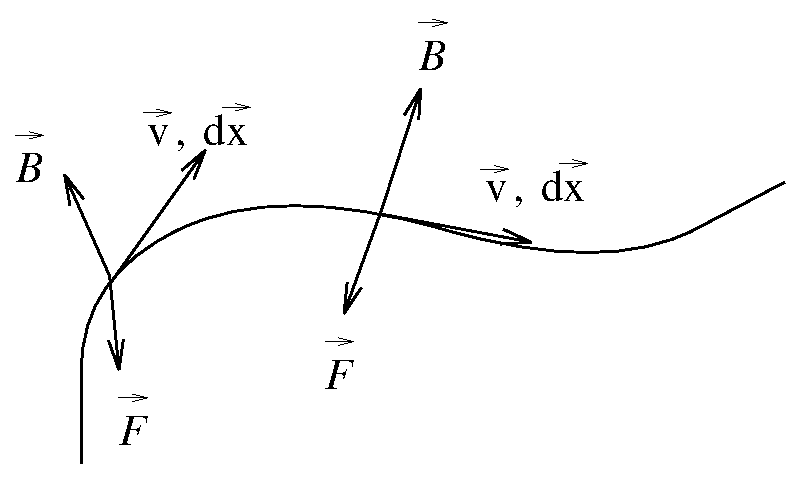
\includegraphics[scale=0.6]{3_electrondynamics/lorentz.eps}
\caption{The magnetic field does no work.}
\label{fig:ed:lorentz}
\end{figure}
Since the velocity vector is always tangent to the particle's path, the 
velocity $\vec{v}$ and the differential element $d\vec{x}$ always point in the 
same direction.  Because of the cross product in~(\ref{eq:ed:lorentz}), the 
force is always perpendicular to the magnetic field $\vec{B}$ and the velocity 
$\vec{v}$; therefore perpendicular to $d\vec{x}$ as well. Hence 
$\vec{F}\cdot d\vec{x}=0$ at every point along the particle's path, so that 
the work done by the field between any two path points 1 and 2 is zero:
$$
W_{\mbox{mag}} = \int_1^2 \vec{F}\cdot d\vec{x}=0.
$$
Since the magnetic field does no work, the kinetic energy of the particle 
cannot change once it passes the anode in Figure~\ref{fig:ed:elec}. 
Remembering the relationship between kinetic energy and velocity, we note that 
the magnitude of the particle's velocity must then be constant.  Therefore: A 
magnetic field can change the {\it direction} of a particle's velocity, but 
not the {\it magnitude} of it's velocity.

This statement becomes more powerful in the case where the magnetic field is
uniform. By uniform, we mean that the field is everywhere in the same 
direction and of constant magnitude.  For the situation at hand, this
amounts to saying that $\vec{B}$ has constant magnitude $B$ and is in the 
-$z$-direction; or simply $\vec{B}=-B\hat{z}$, with $B$ a positive constant. 
If we write out equation~(\ref{eq:ed:lorentz}) in components (note the 
coordinates drawn in Figure~\ref{fig:ed:elec}), we find
\begin{eqnarray*}
F_x &=& -q B v_y \nonumber \\
F_y &=& +q B v_x \\
F_z &=& 0. \nonumber
\end{eqnarray*}
Since the component of force in the $z$-direction is zero, if the particle
starts out with its velocity along the $x$-axis, its motion must be confined
to the $(x,y)$-plane; there's no force to ``push'' it out. The magnitude of
the force
\begin{eqnarray}
|\vec{F}| &=& \sqrt{F_x^2 + F_y^2} \nonumber \\
&=& \sqrt{ \left(qBv_y\right)^2 +  \left(-qBv_x\right)^2 } \nonumber \\
&=& |q|B \sqrt{v_x^2+v_y^2} \nonumber \\
F &=& |q|vB \label{eq:ed:constF}
\end{eqnarray}
is constant since $B$ and $v$ are constant. We have taken the absolute value
of $q$ because the magnitude of the force will always be positive, but the 
charge could be negative. 

A force which is everywhere perpendicular to the motion and of constant 
magnitude is called a {\it centripetal} force. Such a force constrains the 
particle to move in a circle with radius $R$ given by the condition
\begin{equation}
F=\frac{mv^2}{R}. \label{eq:ed:circmot}
\end{equation}   
Figure~\ref{fig:ed:circorb} illustrates the circular path of a negatively 
charged particle (such as an electron) in a uniform magnetic field pointing 
into the page. 
\begin{figure}[htb]
\centering \epsfxsize=7cm 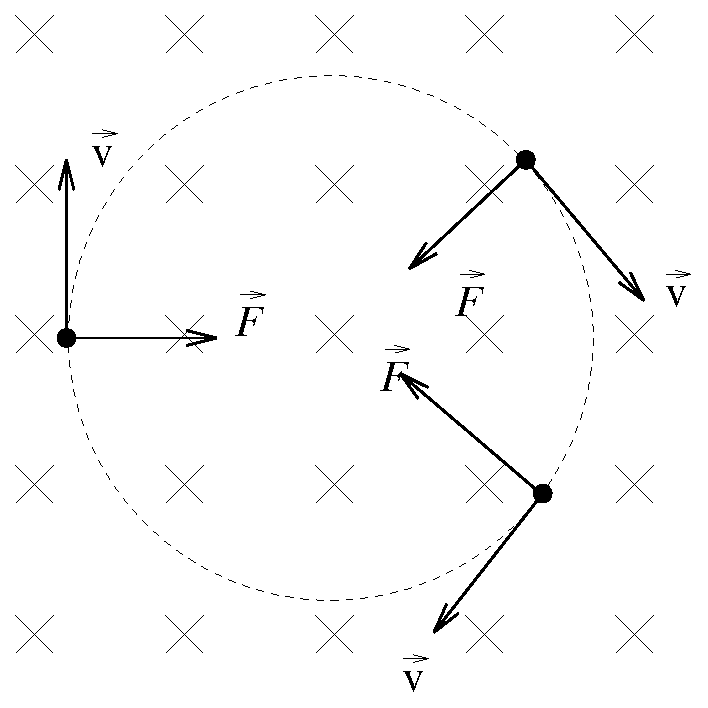
\includegraphics[scale=0.6]{3_electrondynamics/circorb.eps}
\caption{A centripetal force results in a circular orbit.}
\label{fig:ed:circorb}
\end{figure}
A particle with positive charge would move in the opposite 
direction. If we set the expressions for the centripetal 
force~(\ref{eq:ed:constF}) and~(\ref{eq:ed:circmot}) equal to each other, we 
find that the radius of the path is given by
$$
R=\frac{mv}{|q|B}.
$$
The velocity of the particle is just that imparted to it by the accelerating
potential, given by equation~(\ref{eq:ed:velocity}). After some algebra, we 
find
$$
R=\sqrt{\frac{2mV}{|q|B^2}}.
$$
It is easy to see that, as was claimed in the introduction, particles with
different charges will move in circles of different radii.  What happens for
particles of the same charge but different masses?

We can apply this to our particular case, where we only have electrons in our
beam. Electrons all have the same charge, 
$q=-e=-1.602~177~33(49)\cdot 10^{-19}$ C, so that there will be one path, of 
radius 
$$
R=\sqrt{\frac{2mV}{eB^2}}.
$$
We can equivalently write
\begin{equation}
\fbox{$ \displaystyle R^2 = \frac{2mV}{eB^2}$} \label{eq:ed:eoverm}
\end{equation}
which illustrates two important relationships: if we fix $V$, $R^2$ depends 
linearly on the quantity $1/B^2$; if we instead fix $B$, $R^2$ depends linearly
on $V$. In either case, the slope of such a line can be used to obtain the
fundamental quantity we are setting out to measure, the  charge-to-mass ratio of
the electron. The accepted value for this quantity is:
\begin{displaymath}
e/m=1.758~819~62(53)\cdot 10^{11}\rm ~C/kg.
\end{displaymath}

\section{Apparatus}

The apparatus we will use appears in Figure~\ref{fig:ed:apparatus}.
We represent the electron gun schematically in Figure~\ref{fig:ed:electrongun}.
The filament is heated to a temperature in excess of 1500 K. At this 
temperature, electrons are ``boiling'' off of the metal. The electrons are then
accelerated by the electric potential maintained between the anode and the 
filament. This potential may be varied and its value can be read off on the 
voltmeter mounted on the apparatus.  A small hole cut in the anode allows some
of the electrons to pass through, where they are then focused into a beam by a 
set of electrodes. This electron gun is much the same as those in televisions 
and computer monitors. In those, the electrons are focused onto a phosphor 
screen, which emits light which appears as images on the screen. Here we send
our electrons into a magnetic field.
\begin{figure}[htb]
\centering \epsfxsize=8cm 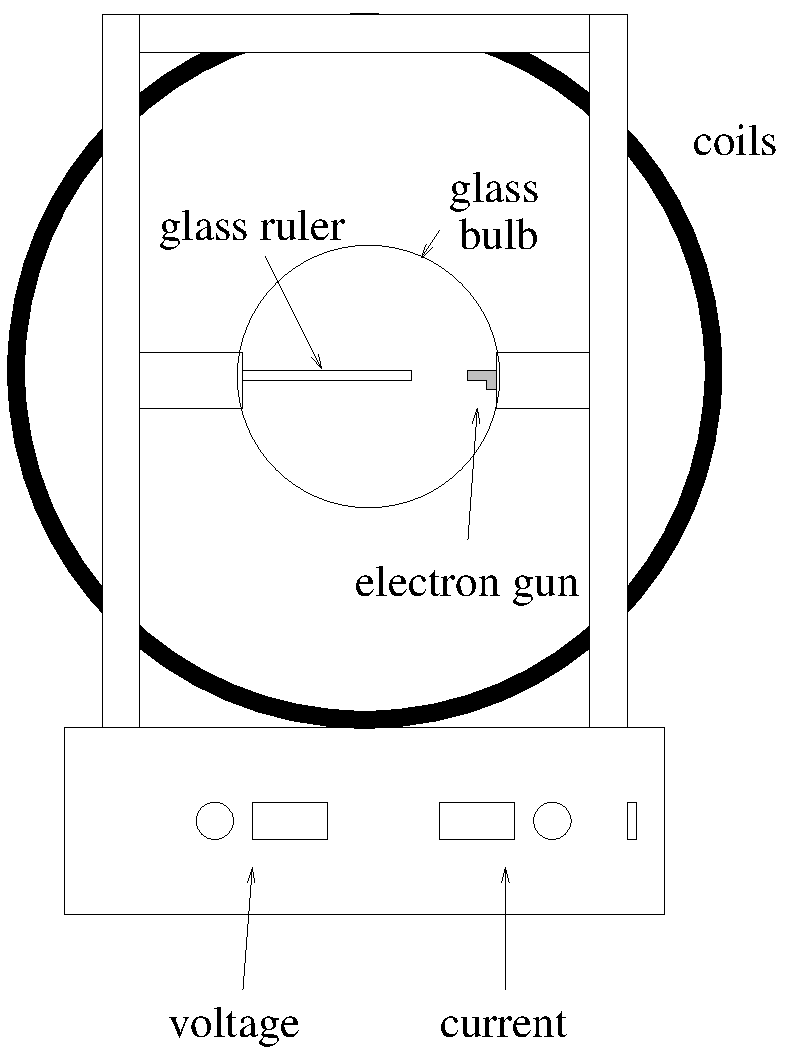
\includegraphics[scale=0.6]{3_electrondynamics/emapparatus.eps}
\caption{The $e/m$ apparatus.}
\label{fig:ed:apparatus}
\end{figure}
\begin{figure}[htb]
\centering \epsfxsize=8cm 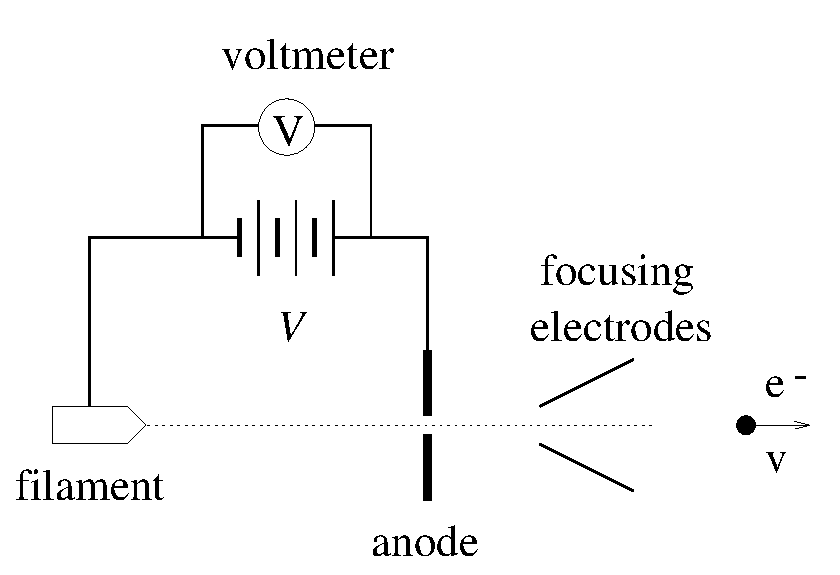
\includegraphics[scale=0.6]{3_electrondynamics/electrongun.eps}
\caption{The electron gun.}
\label{fig:ed:electrongun}
\end{figure}

The electron gun is mounted within a pair of Helmholtz coils, depicted in 
Figure~\ref{fig:ed:helmholtz}.
\begin{figure}[htb]
\centering \epsfxsize=6cm 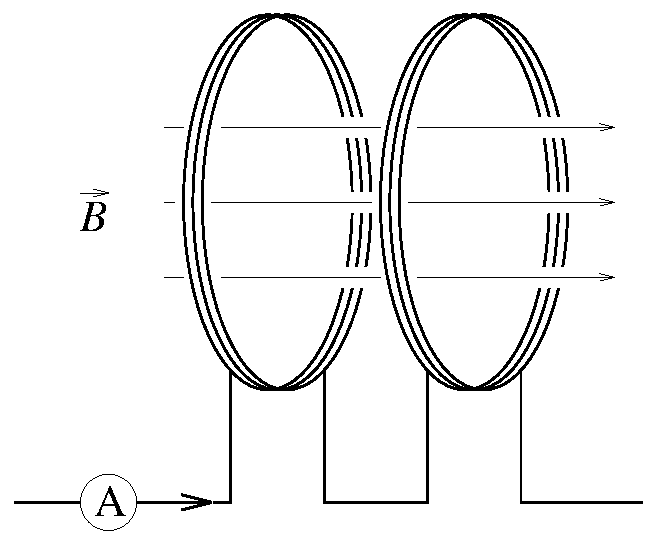
\includegraphics[scale=0.6]{3_electrondynamics/helmholtz.eps}
\caption{Helmholtz coils.}
\label{fig:ed:helmholtz}
\end{figure}
Helmholtz coils are electromagnets in which the magnetic field is extremely 
uniform at the center of the coils; the Helmholtz condition is that the coils 
be separated by a distance equal to their radius.  For the Helmholtz coils on 
the apparatus we're using, you will verify with a compass that the field is 
uniform in the region of the glass bulb, which contains the electron gun. By 
adjusting the current~$I$ through the coils, you can control the magnitude of 
the magnetic field;  the current may be read off of the ammeter mounted on the 
apparatus. If we apply the equation for the magnetic field near the center of 
a coil to our Helmholtz coil apparatus, we find that the magnetic field in the 
region of the bulb may be calculated from the relationship 
\begin{equation}
\fbox{$ \displaystyle B= \left( \frac{4}{5}\right)^{3/2} \frac{\mu_0 N I}{a},$}  
\label{eq:ed:helmB}
\end{equation}
where $N$ is the number of turns in each coil, $a$ is the coil radius, and 
$\mu_0=4\pi\cdot 10^{-7}~\mbox{N/A}^2$. 
 
The glass bulb is filled with helium gas. Some of the electrons in the beam 
collide with the helium atoms; when this happens, the atoms emit blue light.
This light will allow you to see the electron path clearly.  Serway, 
Figure 29.15, p.\ 817, illustrates the blue light quite nicely.  A glass ruler 
mounted inside the bulb allows you to measure the diameter of the 
circular paths, from which you can calculate the radius.

\ \\
\vfill
\pagebreak
$$
$$
\vfill
\clearpage
\newpage

%  Label worksheets by \thechapter.W
\renewcommand{\thesection}{\thechapter.W}

\section{Electron Dynamics Worksheet}
{\bf \Large Name:}~ \rule{5cm}{.1mm}~~~~~~~
{\bf \Large Day/Time:}~\rule{3cm}{.1mm}\\
{\bf \Large Partner's Name:}~\rule{6cm}{.1mm}\\
\subsection{In-Lab Procedure}
\label{sec:ed:proc}

Remember that all measurements and calculations should include units and 
uncertainty.

\subsubsection{The Magnetic Field of the Coils}
\label{sec:ed:bfield}

Measure the radius, $a$, of one of the coils used in the 
apparatus.  (You might find it easier to measure the diameter and then divide 
by 2.) As an estimate of the number of turns in a typical coil, we will take
$$ N = 130 \pm 5. $$  What was 
your measurement of the coil radius with uncertainty? \\
\ \\
\hspace*{5cm} $a$=~\rule{3cm}{.1mm}

\noindent Turn on the apparatus and wait for it to warm up.  Set the current 
through the coils to a moderate value (the maximum 3 A is preferable).  Using
the compass, you will make a rough sketch of the field produced by the coils.
The method is explained now.  
\begin{figure}[htb]
\centering \epsfxsize=5cm 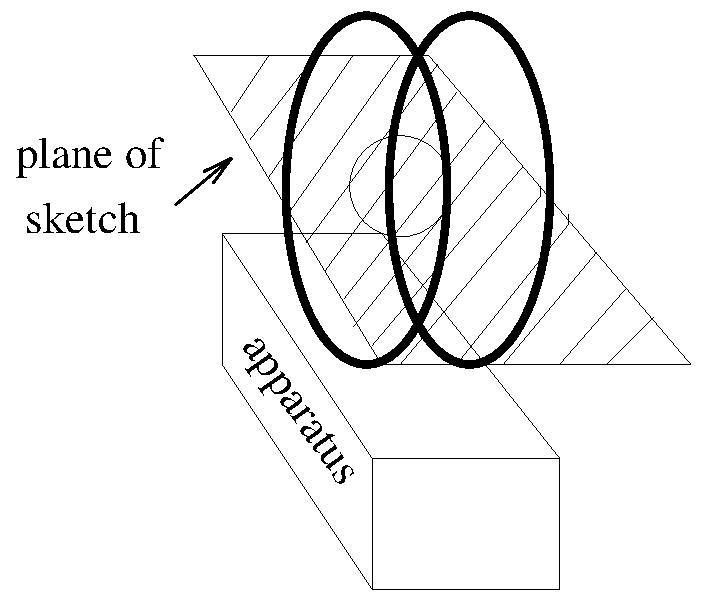
\includegraphics[scale=0.5]{3_electrondynamics/sketch.eps} 
\caption{How to sketch the magnetic field.} 
\label{fig:ed:sketch}
\end{figure}

\begin{figure}[htb]
\centering \epsfxsize=5cm 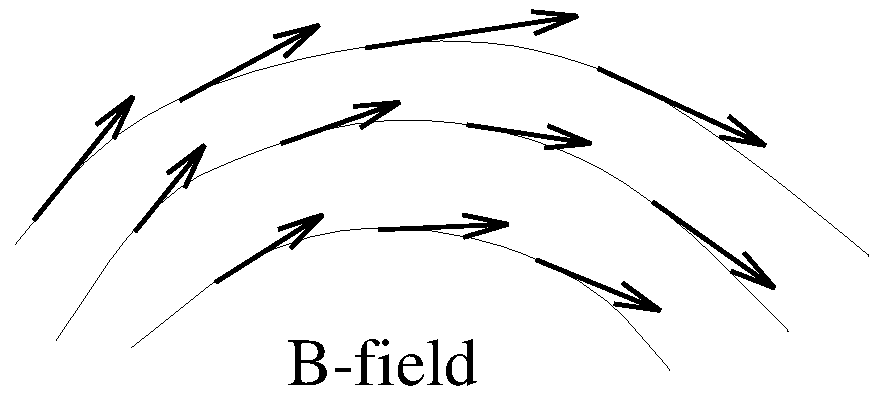
\includegraphics[scale=0.4]{3_electrondynamics/bfield.eps}
\caption{The compass needle points in the direction tangent to the field.}
\label{fig:ed:bfield}
\end{figure}

\noindent Since the Helmholtz coils are cylindrically symmetric, you should
only sketch the field in the plane that forms the horizontal diameter, {\it
i.e.}, as in the Figure~\ref{fig:ed:sketch}. The {\it compass needle will point
in the direction tangent to the field}, as in Figure~\ref{fig:ed:bfield}.
By sketching the compass directions as small arrows on paper, 
you can trace out the field lines by using the arrows as tangents to the
curves. You should do this in {\it pencil}.  When sketching the field lines,
pay particular attention to the region of the glass bulb.  
Use Figure~\ref{fig:ed:worksketch} to make your sketch of the magnetic field. 
This figure is from the viewpoint of looking down at the coils.  Draw
on Figure~\ref{fig:ed:worksketch} now.


\begin{figure}[!htb]
\vspace*{1.9cm}
\centering
\epsfxsize=6cm 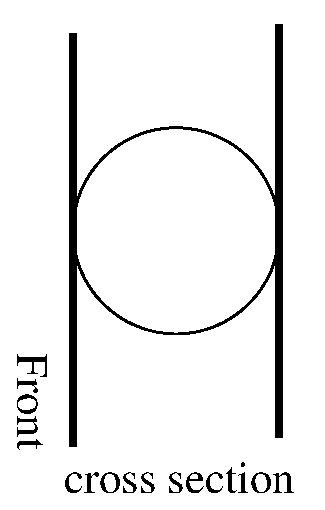
\includegraphics[scale=0.6]{3_electrondynamics/csect.eps}
\vspace*{2cm}
\caption{\textbf{Sketch the magnetic field in this cross-section picture.}} 
\label{fig:ed:worksketch}
\end{figure}

\vfill 
\newpage

\subsubsection{Radius versus Magnetic Field}
\label{sec:ed:varyB}

Set the accelerating voltage $V$ to 300 V and measure the electron 
path radius $R$ as a function of the magnetic field $B$ by varying the coil 
current $I$.  Remember that what you actually measure with the apparatus is
the diameter. You will need to calculate the radius yourself. The 
magnetic field is calculated from equation~(\ref{eq:ed:helmB}) and the 
information gathered in $\S$~\ref{sec:ed:bfield}. 
Enter your 8 sets of data for current and radius (note that the ruler
in the glass bulb measures diameter) into Table~\ref{tab:ed:varyb} with
{\bf units and uncertainties}.\\

\hspace{3cm} Accelerating Voltage $V$ =~\rule{3cm}{.1mm}  


\begin{table}[htb]
\begin{center}
\begin{tabular}{|c|c|}
\hline
\multicolumn{2}{|c|}{Varied Current}\\
\hline
I & R \\
\hline
\hspace*{5cm} & \hspace*{5cm} \\
& \\
\hline       
& \\
& \\
\hline
& \\
& \\
\hline
& \\
& \\
\hline
& \\
& \\
\hline
& \\
& \\
\hline
& \\
& \\
\hline
& \\
& \\
\hline
\end{tabular}
\end{center}
\caption{I and R for varying magnetic field.}
\label{tab:ed:varyb}
\end{table}

\noindent For the digital displays only, you may take the 
uncertainty to be a one in the last decimal place. For example, if you read a 
voltage as 142~V, then the uncertainty is 1~V.  Report the measurement in 
the proper form; for the example, this would be $142 \pm 1$~V. You must 
estimate the uncertainty in the diameter measurement yourself. Be sure to take 
into account the precision with which you can read the scale and the width of 
the electron beam when doing this. 
 
\subsection{In-Lab Computer Work}
You are now going to plot $R^2 \mbox{ vs. } 1/B^2$ and fit the line.  
Remember from the computer 
introduction classes that you can have the computer do most of the work
for you.  You can just enter the coil radius value 
from $\S$~\ref{sec:ed:bfield}, the current values, the path radius values, and 
all of the associated uncertainties into the computer; it will do all of the 
necessary calculations (calculate $B$, etc.) to give you this graph and will 
calculate the slope and $R^2$ intercept using a linear least squares routine.\\
\ \\
\noindent {\bf The uncertainty for this graph is $\Delta(B^{-2})$.}  Perform 
the following calculations to help you get through the calculation of 
$\Delta(B^{-2})$. \\
\ \\
\noindent Write down the formula for $B$. \\
\vspace*{1cm} \\
\hspace*{5cm} $B$ = \\
\ \\
\noindent Plug in your first set of numbers from Table~\ref{tab:ed:varyb} 
and the constants to calculate a number for $B$ now. \\
\vspace*{1cm} \\           
\hspace*{5cm} $B$ =~\rule{3cm}{.1mm}\\ 
\noindent Calculate $\Delta(B)$ {\bf without numbers}. Show work. \\
\vspace*{3cm} \\
\hspace*{5cm} $\Delta(B)$ = \\
\ \\
%\newpage
\noindent Plug in your first set of numbers to calculate a  number for 
$\Delta(B)$ now.\\
\vspace*{1cm} \\
\hspace*{5cm} $\Delta(B)$ =~\rule{3cm}{.1mm} \\
\ \\
\noindent Calculate $\Delta(B^{-2})$ {\bf without numbers}. Show work.
Hint: You already know $B$ and $\Delta(B)$.  \\
\vspace*{3cm} \\
\hspace*{5cm} $\Delta(B^{-2})$ = \\
\ \\
\noindent Plug in your first set of numbers to calculate a  number for 
$\Delta(B^{-2})$ now.  \\
\vspace*{1cm} \\
\hspace*{5cm} $\Delta(B^{-2})$ =~\rule{3cm}{.1mm} \\
\ \\
\noindent Now you can plug in the equation for $B$ and $\Delta(B^{-2})$
into Kaleidagraph.  You also have already done a sample
calculation.   {\bf Always do a sample calculation
to check the validity of what you typed into the computer.}  Now plot
$R^2 \mbox{ vs. } 1/B^2$ and fit the line.
Write down the slope (with units and uncertainty) below. \\
\ \\
\hspace*{5cm} $S_1$ =~\rule{3cm}{.1mm}\\ 
\ \\
\noindent From equation~(\ref{eq:ed:eoverm}) the slope of the line should be $$S_1=\frac{2Vm}{e}.$$


\subsection{In-Lab Procedure}
\subsubsection{Radius versus Potential}
\label{sec:ed:pot}

Now set the coil current to a fixed value (about 2 A) and measure the 
path radius as a function of the accelerating potential for at least 
8 data points.  Enter your data for voltage and radius into 
Table~\ref{tab:ed:pot}.  Remember
your units and uncertainties.\\

\hspace{3cm} Current Setting  $I$=~\rule{3cm}{.1mm}

\begin{table}[htb]
\begin{center}
\begin{tabular}{|c|c|}
\hline
\multicolumn{2}{|c|}{Varied Voltage}\\
\hline
V & R \\
\hline
\hspace*{5cm} & \hspace*{5cm} \\
& \\
\hline       
& \\
& \\
\hline
& \\
& \\
\hline
& \\
& \\
\hline
& \\
& \\
\hline
& \\
& \\
\hline
& \\
& \\
\hline
& \\
& \\
\hline
\end{tabular}
\end{center}
\caption{V and R for varying voltage.}
\label{tab:ed:pot}
\end{table}

\subsection{In-Lab Computer Work}
Plot $R^2 \mbox{ vs. } V$ and fit the line.  
Write down the slope (with units and uncertainty) below. \\
\ \\
\hspace*{5cm} $S_2$ =~\rule{3cm}{.1mm}\\ 
\ \\
\noindent Also from equation~(\ref{eq:ed:eoverm}) we have that
the slope of this line should be
$$S_2=\frac{2m}{eB^2}.$$
 
\subsection{Pre-Classroom Check List}
\noindent This check list is intended to be a guide for 
you to prepare yourself 
for the classroom work.  You cannot come back to lab during this hour,
collaborate with colleagues, nor hand in the worksheet late.  Make sure
you have completed everything.  
\vskip \baselineskip
\noindent {\bf Pre-classroom Check List}  
\vskip\baselineskip
\noindent $\bigcirc$ \hspace*{1cm} Table~\ref{tab:ed:varyb} completed with units and uncertainties \\
$\bigcirc$ \hspace*{1cm} Table~\ref{tab:ed:pot} completed with units and uncertainties \\
$\bigcirc$ \hspace*{1cm} $S_1$ with uncertainty and units \\
$\bigcirc$ \hspace*{1cm} $S_2$ with uncertainty and units \\
$\bigcirc$ \hspace*{1cm} 2 Plots labeled completely and correctly \\
$\bigcirc$ \hspace*{1cm} Each student has her/his own plots and worksheet \\
 

\subsection{In-Classroom Calculations $\&$ Analysis}
\subsubsection{The Magnetic Field of the Coils}
%\noindent What is the magnetic field like inside the glass bulb? \\
%\vspace*{2cm} \\
\noindent Is the magnetic field uniform inside the glass bulb? \\
\vspace*{1.0cm} \\

\noindent From the direction of the electron velocity and the centripetal force,
determine the direction of the magnetic field inside the glass bulb.
Does this agree with your drawing in Figure~\ref{fig:ed:worksketch}.\\
\vspace*{1cm} \\

\subsubsection{Radius versus Magnetic Field}
\noindent Using the slope $S_1$ and $V$ with their uncertainties, calculate a
value for $e/m$ and its uncertainty.  {\bf SHOW WORK.}\\ 
\vspace*{6cm}\\
\hspace*{2cm} {$(e/m)_1$ =~\rule{3cm}{.1mm}}\\ 

\subsubsection{Radius versus Potential}
\noindent Using the slope $S_2$ and $B$ ({\it note that you have to calculate 
the latter}) with their uncertainties, calculate a value for $e/m$ and its
uncertainty. {\bf SHOW WORK.}\\ 
\vspace*{6cm}\\
\hspace*{2cm} {$(e/m)_2$ =~\rule{3cm}{.1mm}}\\ 

\subsection{In-Classroom Discussion}
\noindent Compare both values of $e/m$ you measured to the accepted value
$1.758~819~62(53)\cdot 10^{11}$~C/kg, as well as to each other. Also compare
your observations and the results of your analysis with the objectives set out
for the lab in the introduction, Section~\ref{sec:ed:intro}. Did you observe 
everything you expected?  Do this in the space provided.  You may write on
the back of this page if necessary or staple a labeled extra sheet. 


\vfill
\noindent Attach plots to the worksheet. \\
\ \\
{\Large End Worksheet} 

% Go back to ordinary section numbering
\renewcommand{\thesection}{\thechapter.\arabic{section}}























